% Demo: the Homework preset in Overleaf's default article at 11 pt (no geometry: \linewidth = 360pt)
\documentclass[11pt]{article}
\usepackage[T1]{fontenc}
\usepackage{lmodern}
\usepackage{graphicx,amsmath,amssymb,float}
\graphicspath{{../out/}}
\begin{document}
\noindent\textbf{Problem 2.} Find a M\"obius map that sends $0,1,\infty$ to $1,i,-1$.

\medskip\noindent\textit{Solution.} A short solution stands here. The figure of the next problem must not float above it.

\bigskip\noindent\textbf{Problem 3.} Show that $F(z)=\dfrac{z-i}{z+i}$ maps the upper half-plane $\mathbb{H}$ conformally onto the unit disk $\mathbb{D}$.

\medskip\noindent\textit{Solution.} For real $x$ we have $|x-i|=|x+i|$, so $F$ maps $\mathbb{R}$ into the unit circle; since $F(i)=0\in\mathbb{D}$ and $\mathbb{H}$ is connected, $F(\mathbb{H})=\mathbb{D}$. In Figure~\ref{fig:cayley-hw}, walking along $\mathbb{R}$ from $A$ to $C$ keeps $\mathbb{H}$ on the left, and its image keeps $\mathbb{D}$ on the left.

% cayley-hw.pdf is made for \linewidth = 360pt (article, 11pt, default margins); natural size wherever it fits.
% Preamble: \usepackage{graphicx,amsmath,amssymb,float}
\begin{figure}[H]
  \centering
  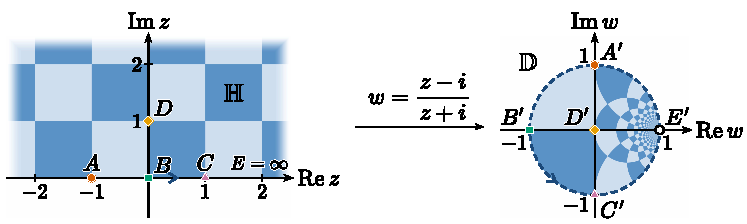
\includegraphics[width=\ifdim\linewidth<360pt \linewidth\else 360pt\fi]{cayley-hw}
  \caption{$w=(z-i)/(z+i)$ on $\mathbb{H}$: the points $A$--$E$ and their images $A'$--$E'$. Dashed: boundary not included; arrowheads: orientation.}
  \label{fig:cayley-hw}
\end{figure}

The figure stays here, right after the solution that cites it.
\end{document}
